\documentclass[tikz,border=5pt]{standalone}

\usepackage{fontspec}
\usepackage{unicode-math}
\usepackage{pgfplots}

\pgfplotsset{compat=1.18}

% Compile with LuaLaTeX or XeLaTeX.
\setmainfont{STIX Two Text}
\setmathfont{STIX Two Math}

\colorlet{functioncolor}{red!75!black}
\colorlet{rulecolor}{blue!65!black}

\begin{document}

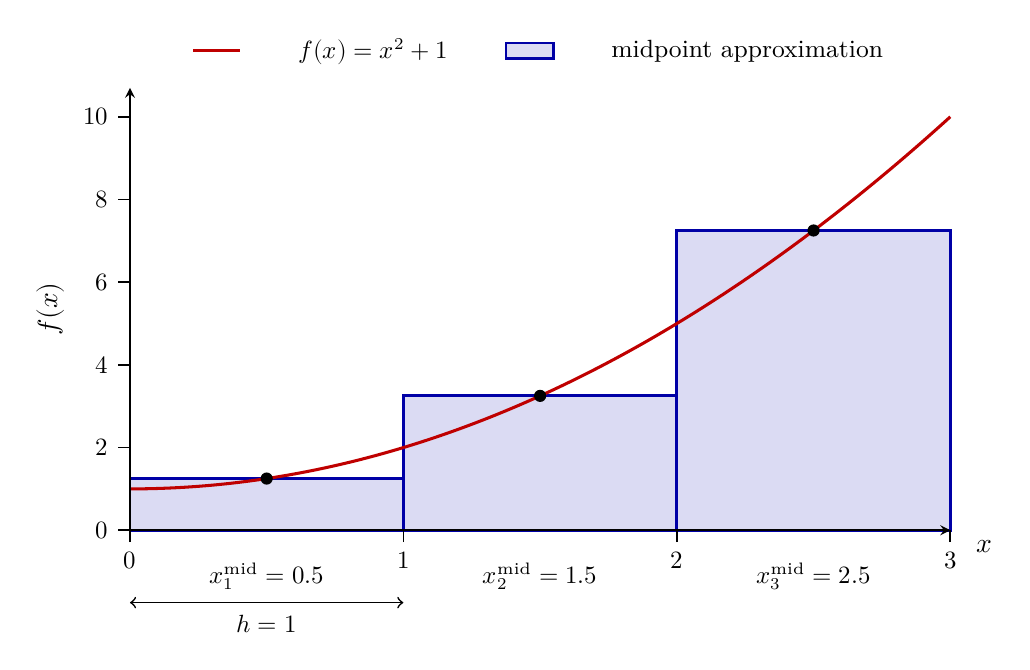
\begin{tikzpicture}

  \begin{axis}[
      width=12cm,
      height=7.2cm,
      xmin=0, xmax=3,
      ymin=0, ymax=10.7,
      axis lines=left,
      axis on top,
      axis line style={black, semithick},
      tick align=outside,
      tick style={black, semithick},
      xlabel={\(x\)},
      ylabel={\(f(x)\)},
      xlabel style={at={(axis description cs:1.02,0)}, anchor=north west},
      xtick={0,1,2,3},
      ytick={0,2,4,6,8,10},
      tick label style={font=\small},
      label style={font=\normalsize},
      legend style={
          at={(0.5,1.03)},
          anchor=south,
          draw=none,
          fill=none,
          font=\small,
          legend columns=-1,
          column sep=0.65cm,
        },
      clip=false,
    ]

    % Midpoint rectangles, drawn first so the function remains visible.
    \fill[rulecolor!14] (axis cs:0,0) rectangle (axis cs:1,{0.5^2+1});
    \fill[rulecolor!14] (axis cs:1,0) rectangle (axis cs:2,{1.5^2+1});
    \fill[rulecolor!14] (axis cs:2,0) rectangle (axis cs:3,{2.5^2+1});

    \draw[rulecolor, line width=1pt] (axis cs:0,0) rectangle (axis cs:1,{0.5^2+1});
    \draw[rulecolor, line width=1pt] (axis cs:1,0) rectangle (axis cs:2,{1.5^2+1});
    \draw[rulecolor, line width=1pt] (axis cs:2,0) rectangle (axis cs:3,{2.5^2+1});

    % The integrand.
    \addplot[
      domain=0:3,
      samples=150,
      functioncolor,
      line width=1.1pt,
      forget plot,
    ] {x^2+1};

    % Midpoint evaluation points.
    \fill[black] (axis cs:0.5,{0.5^2+1}) circle (2.2pt);
    \fill[black] (axis cs:1.5,{1.5^2+1}) circle (2.2pt);
    \fill[black] (axis cs:2.5,{2.5^2+1}) circle (2.2pt);

    % Midpoint labels form a separate row below the numerical tick labels.
    \node[anchor=north, font=\small] at (axis cs:0.5,-0.55)
    {\(x_1^{\mathrm{mid}}=0.5\)};
    \node[anchor=north, font=\small] at (axis cs:1.5,-0.55)
    {\(x_2^{\mathrm{mid}}=1.5\)};
    \node[anchor=north, font=\small] at (axis cs:2.5,-0.55)
    {\(x_3^{\mathrm{mid}}=2.5\)};

    % One dimension line to identify the uniform spacing.
    \draw[<->, semithick]
    (axis cs:0,-1.75) -- (axis cs:1,-1.75)
    node[midway, below=1pt, font=\small] {\(h=1\)};

    % Compact two-item legend, shared in style with the trapezoidal figure.
    \addlegendimage{functioncolor, line width=1.1pt}
    \addlegendentry{\(f(x)=x^2+1\)}
    \addlegendimage{area legend, draw=rulecolor, fill=rulecolor!14, line width=1pt}
    \addlegendentry{midpoint approximation}

  \end{axis}

\end{tikzpicture}

\end{document}
